\documentclass[UTF8]{ctexart}
\usepackage{CJKutf8}
\usepackage{listings}
\usepackage{geometry}
\usepackage{xcolor}
\usepackage{graphics}
\usepackage{graphicx}
\lstset{
	backgroundcolor=\color{white},
	basicstyle=\footnotesize\ttfamily,
	breakatwhitespace=false,
	breaklines=true,
	captionpos=b,
	commentstyle=\color{mygreen},
	deletekeywords={...},
	escapeinside={\%*}{*)},
	extendedchars=true,
	frame=single,
	keepspaces=true,
	keywordstyle=\color{blue},
	morekeywords={*,...},
	numbers=left,
	numbersep=5pt,
	numberstyle=\tiny\color{gray},
	rulecolor=\color{black},
	showspaces=false,
	showstringspaces=false,
	showtabs=false,
	stepnumber=4,
	stringstyle=\color{purple},
	tabsize=4,
	title=\lstname
}
\geometry{a4paper, left=1cm, right=1cm, bottom=1cm}
\title{操作系统实验报告}
\author{顾芃骐20079100001}
\begin{document}
	\maketitle
	\newpage
	\section{进程的建立}
	\begin{itemize}
		\item 实验目的:学会通过基本的Windows或者Linux进程控制函数,由父进程创建子进程,并实现父子进程协同工作。
		\item 实验软件环境:Ubuntu22.04 \& GNU-C++17
		\item 实验内容:创建两个进程,让子进程读取一个文件,父进程等待子进程读取完文件后继续执行,实现进程协同工作。进程协同工作就是协调好两个进程,使之安排好先后次序并以此执行,可以用等待 函数来实现这一点。当需要等待子进程运行结束时,可在父进程中调用等待函数。
	\end{itemize}
	\subsection{代码实现}
    在“\textbf{\textit{os1.cpp}}”中写如下代码,并创建名为“\textbf{\textit{os1.in}}”的文件,在后者中写入且仅写入“TextMessage”作为测试输出内容。
\begin{lstlisting}[language=c++]
#include<fstream>
#include<unistd.h>
#include<stdio.h>
#include<iostream>
using namespace std;
int main(){
	int flag = 0;
	string answer = "";
	auto x = vfork();
	if (!x) {
		ifstream in("os1.in");
		in >> answer;
		in.close();
		flag = 1;
		cout << "End of Child Process" << endl;
	} else {
		while (!flag);
		cout << "Start of Main Process" << endl;
		cout << answer << endl;
		cout << "End of Main Process" << endl;
	}
	return EXIT_SUCCESS;
}
\end{lstlisting}
\subsection{实验结果}
运行上述代码,可得到如下左图所示的实验结果。片刻之后,终端显示如右所示的结果。
\begin{center}
        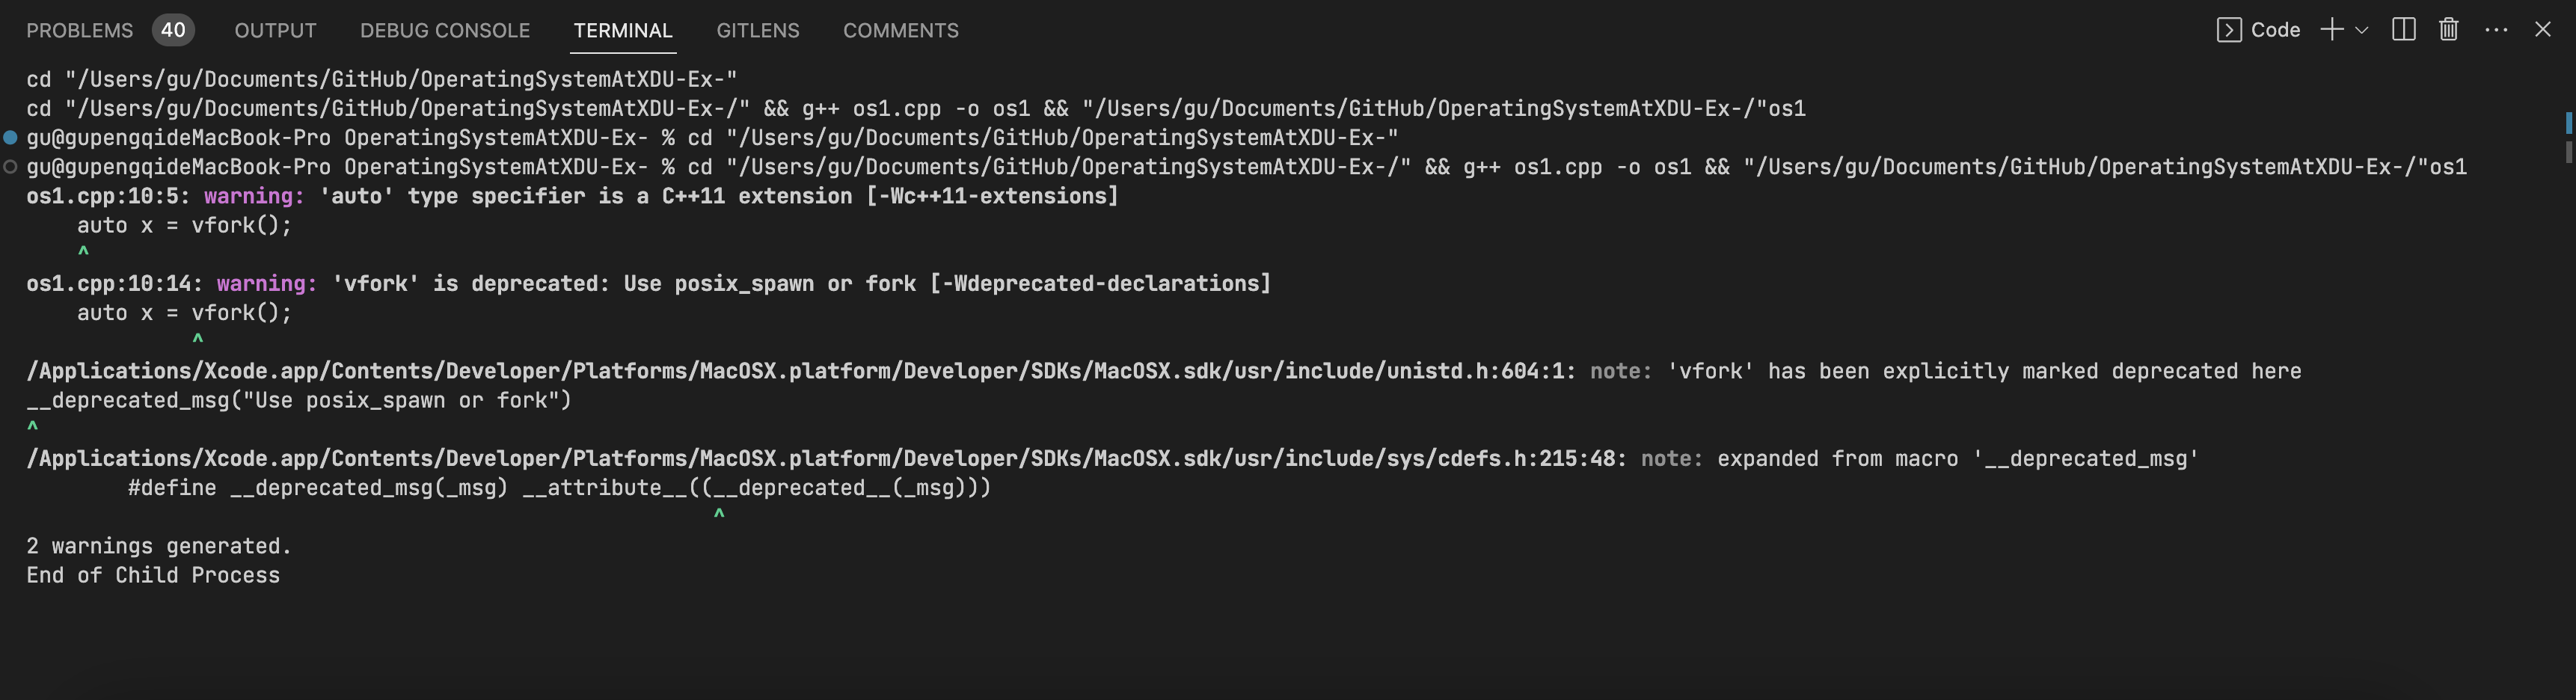
\includegraphics[width=0.3\pdfpagewidth]{os1-1.png}
        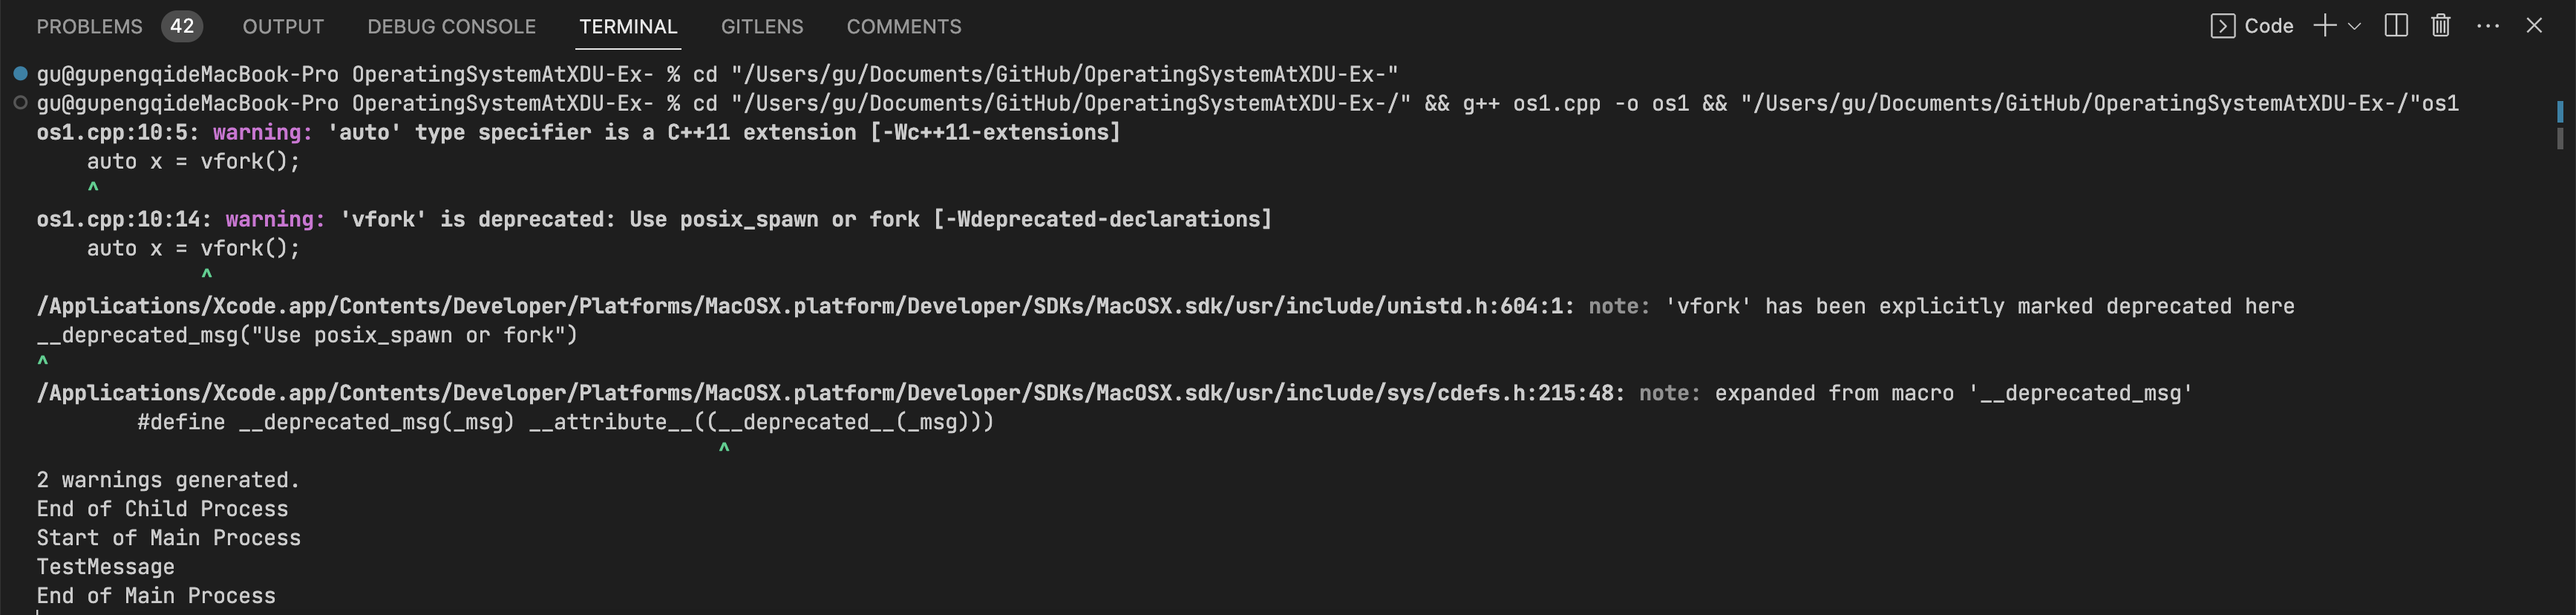
\includegraphics[width=0.3\pdfpagewidth]{os1-2.png}
\end{center}
\subsection{实验结果分析}
在1.1所示代码中,子进程读取了文件“\textit{os1.in}”;读取完成后,父进程继续执行,并显示了开始、结束和子进程所读取的文件内容。需要注意的是,使用\texttt{vfork}时修改静态区变量是未定义行为,会引发“栈溢出(stack smashing)”。
\section{线程共享进程数据}
\begin{itemize}
	\item 实验目的:了解线程与进程之间的数据共享关系。创建一个线程,在线程中更改进程中的数据。
	\item 实验软件环境: Ubuntu22.04 \& gnu-c++17
	\item 实验内容: 在进程中定义全局共享数据,在线程中直接引用该数据进行更改并输出该数据。
\end{itemize}
\subsection{代码实现}
在“\textbf{\textit{os2.cpp}}”中写如下代码。
\begin{lstlisting}[language=c++]
#include <thread>
#include <mutex>
#include <bits/stdc++.h>
#include <unistd.h>
using namespace std;
static int Sample = 1;
mutex mutx;
void thread1(int n){
	while (Sample <= n)
	{
		if (mutx.try_lock())
		{
			cout << "Thread1 " << Sample << "\n";
			sleep(1);
			Sample++;
			mutx.unlock();
		}
	}
}
int main(){
	int n = 20;
	thread t1(thread1, n);
	while (Sample <= n){
		if (mutx.try_lock()){
			cout << "MainThread " << Sample << "\n";
			Sample++;
			mutx.unlock();
		}
	}
	return 0;
}
	\end{lstlisting}
\subsection{实验结果}
运行上述代码,可得到实验结果如下图所示。
\begin{figure}
	\begin{center}
		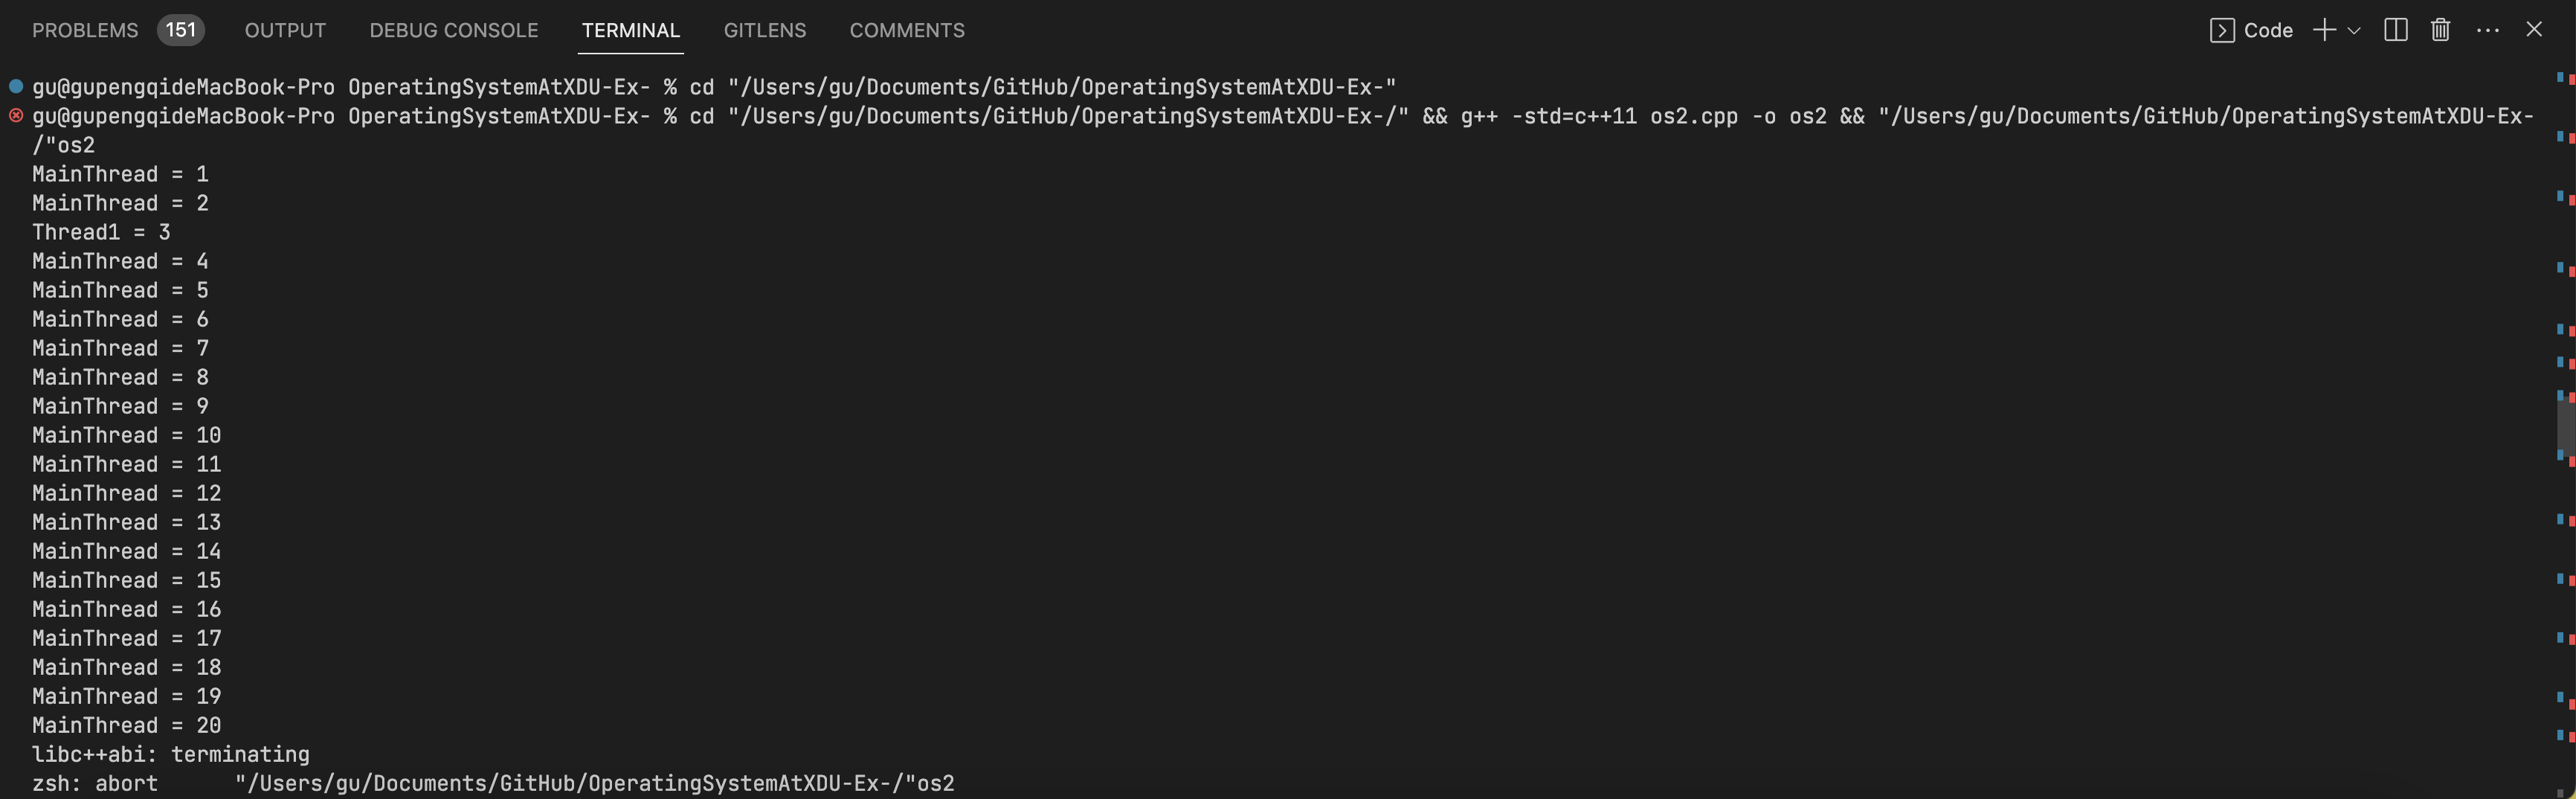
\includegraphics[width=0.7\pdfpagewidth]{os2.png}
	\end{center}
\end{figure}
\subsection{实验结果分析}
在此次实验结果中,当\texttt{Sample}值为3时,执行了\texttt{thread1}函数。线程中直接引用了这一数据进行更改并输出之。
\subsection{反思}
本次实验代码中运行结果可能与“实验结果”章节中的不一致,有时会出现\texttt{thread1}函数不执行的情况,20个输出结果均为“MainThread=x”。
\clearpage
\section{信号通信}
\begin{itemize}
	\item 实验目的:利用信号通信机制在父子进程及兄弟进程间进行通信。
	\item 实验软件环境: Ubuntu22.04 \& gnu-c++17
	\item 实验内容: 父进程创建一个有名事件,由子进程发送事件信号,父进程获取事件信号后进行相应的处理。
\end{itemize}
\subsection{代码实现}
\begin{lstlisting}[language=c++]
#include<unistd.h>
#include<stdlib.h>
#include<signal.h>
#include<bits/stdc++.h>

using namespace std;

void sig_handle(int sig) {
	cout << "Sigint get!\n";
	signal(SIGINT, SIG_DFL);
}
	
int main() {
	auto fa = getpid();
	auto x = fork();
	if( getpid() == fa ) {
		cout << "fa : " << getpid() << "\n";
		if(signal(SIGINT, sig_handle) == SIG_ERR) {
			cout << "ERROR!\n";
		}
		sleep(100);
	} else {
		cout << "ch : " << getpid() << "\n";
		kill( getppid(), SIGINT );
	} 
}
\end{lstlisting}
\subsection{实验结果}
运行上述代码,可得到如下图所示的实验结果。
\begin{figure}[htbp]
	\begin{center}
		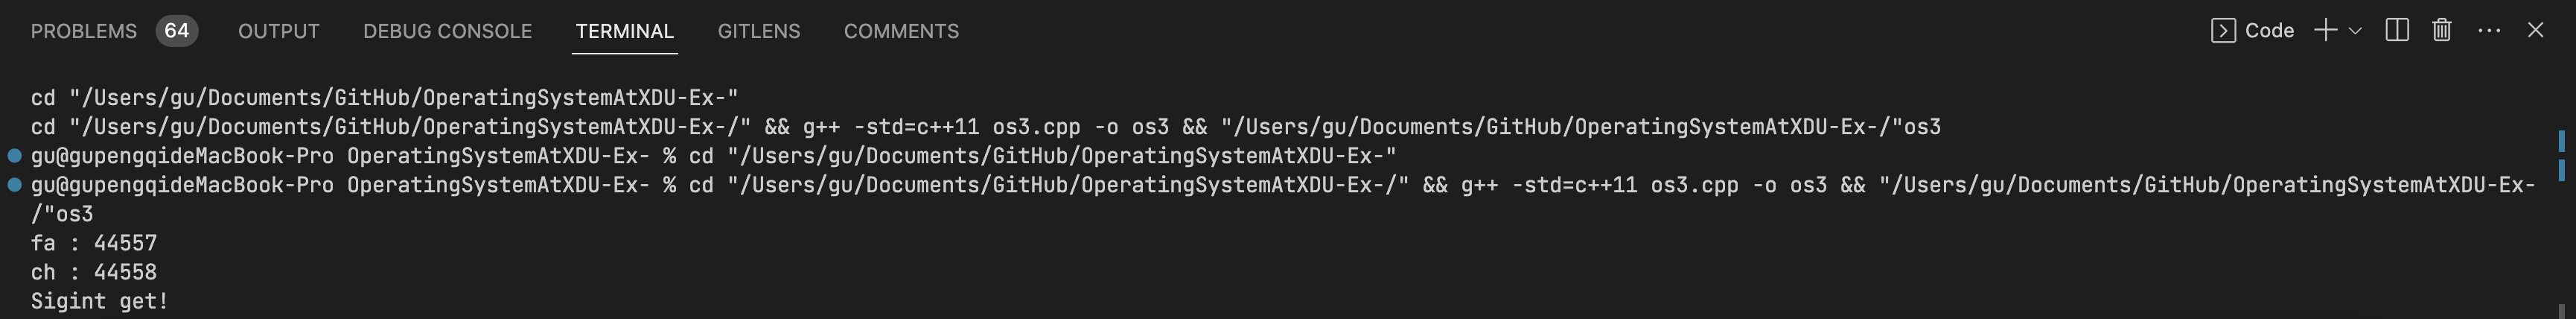
\includegraphics[width=0.8\pdfpagewidth]{os3-1.png}
	\end{center}
\end{figure}
\subsection{实验结果分析}
父进程\texttt{getpid}创建了一个有名事件,由子进程\texttt{ch}完成后发送事件信号,父进程获取这一事件信号后进行相应的处理,反馈为“\textit{Sigint get!}”。\\
每一次运行此代码得到的\texttt{fa}与\texttt{ch}值均不相同。例如,在上方实验结果之后重新运行此程序,得到“\texttt{fa : 47122}”“\texttt{ch : 47123}”和“\textit{Sigint get!}”(下图)。然而所有的运行结果中,\texttt{fa}与\texttt{ch}的值均满足规律
\begin{equation}
	fa + 1 = ch
\end{equation}
这是因为,代码中fa有关输出和ch有关输出总是在同一个条件语句中执行的。
\begin{figure}[htbp]
	\begin{center}
		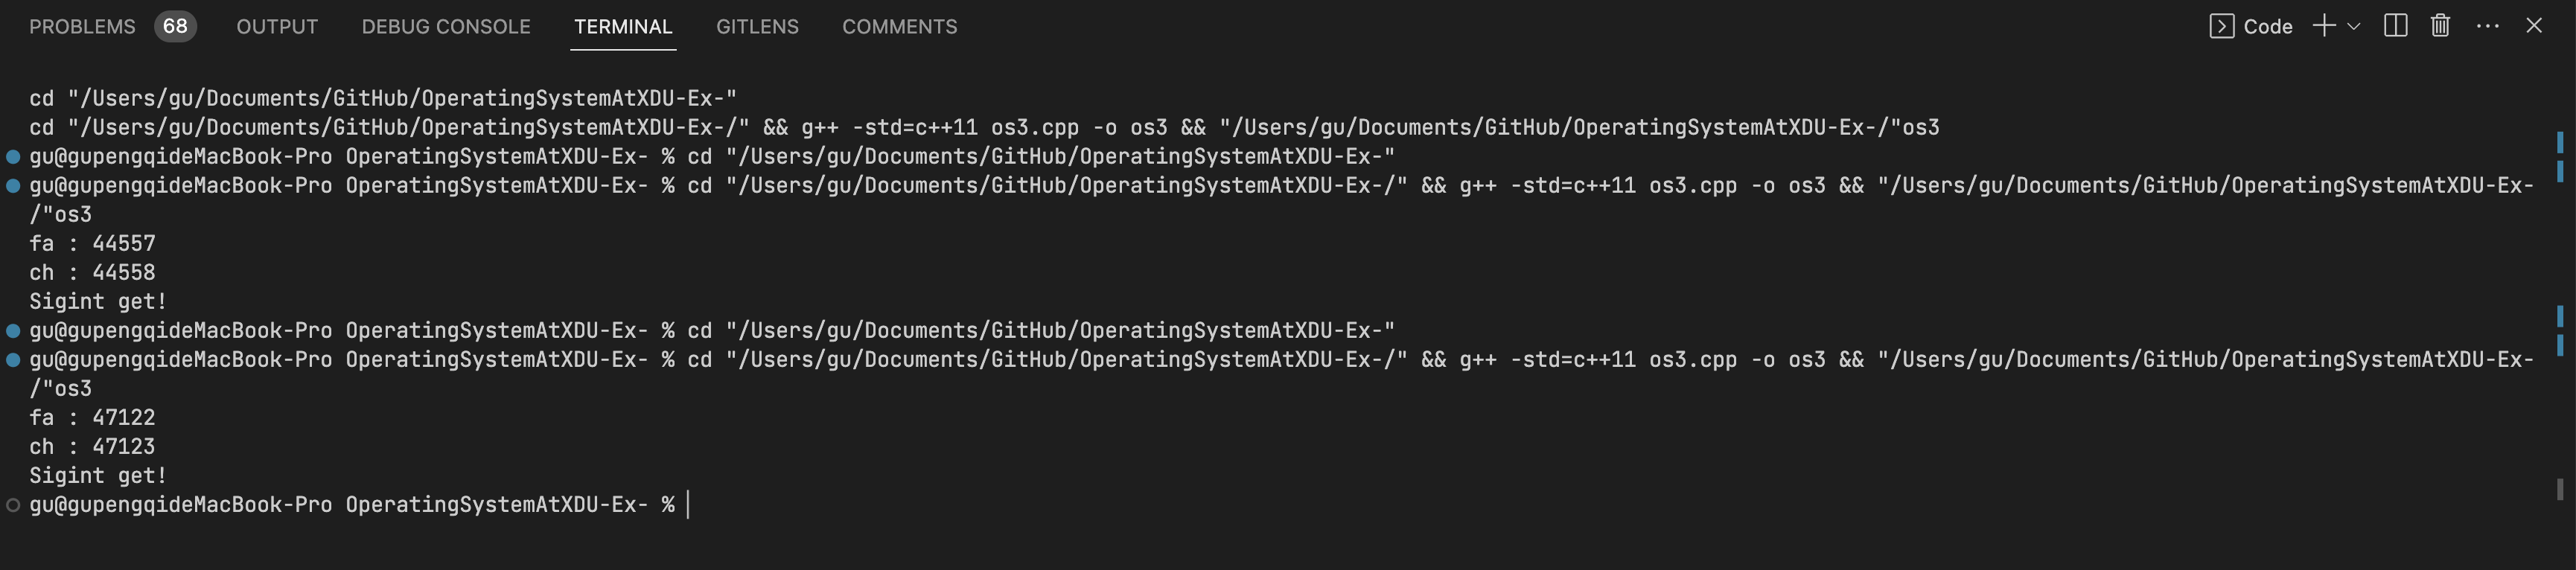
\includegraphics[width=0.8\pdfpagewidth]{os3-2.png}
	\end{center}
	\caption{重新运行此代码,得到的\texttt{fa}与\texttt{ch}数值并不相同}
\end{figure}
\subsection{反思·心得}
信号通信处理是一种很有效的异步处理方式;从此次实验结果来看运行速度很快。
\clearpage
\section{匿名管道通信}
\begin{itemize}
	\item 实验目的:学习使用匿名管道在两个进程间建立通信。
	\item 实验软件环境:Ubuntu22.04 \& gnu-c++17
	\item 实验内容: 分别建立名为 Parent 的单文档应用程序和 Child 的单文档应用程序作为父子进程,由父进程创建一个匿名管道,实现父子进程向匿名管道写入和读取数据。
\end{itemize}
\subsection{代码实现}
\begin{lstlisting}[language=c++]
#include<unistd.h>
#include<bits/stdc++.h>
using namespace std;

int main() {
	auto fa = getpid();
	int _pipeline[2];
	int ret = pipe(_pipeline);
	if(ret < 0) {
		cout << "Pipeline error!\n";
		return 0;
	}
	auto x = fork();
	if( x == 0 ) {
		close(_pipeline[1]);
		char s[100];
		memset(s, '\0', sizeof(s));
		read(_pipeline[0], s, sizeof(s));
		cout << "fa : " << getpid() <<  " reading " << s << "\n";
	}else {
		close(_pipeline[0]);
		char* msg = NULL;
		msg = "TestMessage";
		write(_pipeline[1], msg, strlen(msg));
		cout << "ch : " << getpid() << " Write success!\n";
	} 
	return 0;
}
\end{lstlisting}
\subsection{实验结果}
运行上述代码,可得到如下图所示的实验结果。
\begin{figure}[htbp]
	\begin{center}
		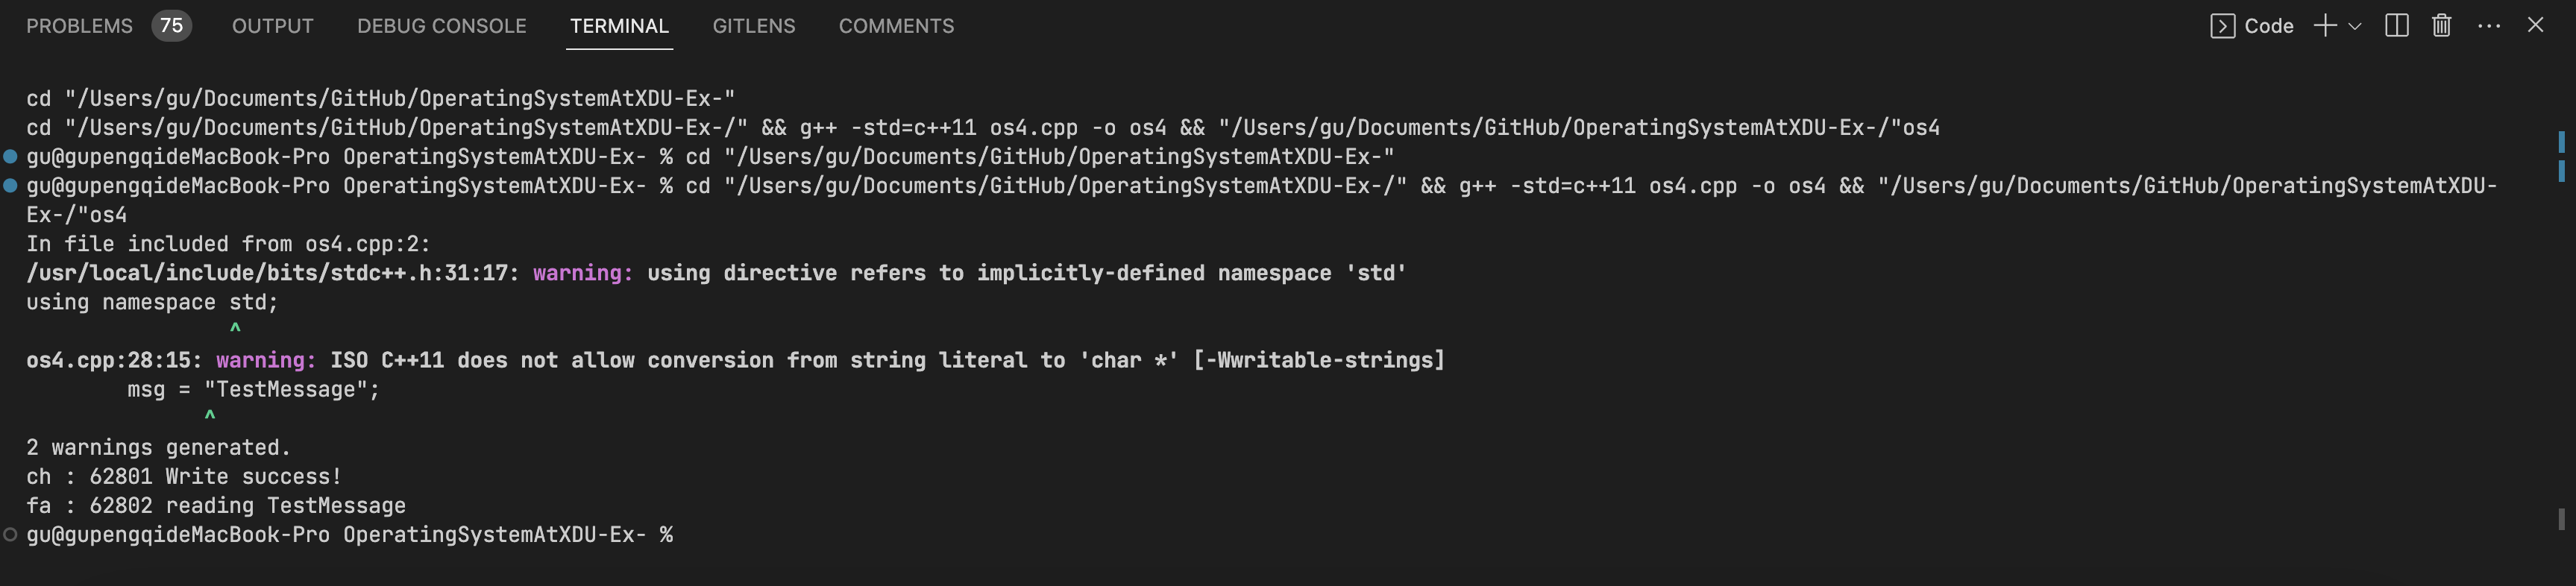
\includegraphics[width=0.8\pdfpagewidth]{os4.png}
	\end{center}
\end{figure}
\subsection{实验结果分析}
父进程\texttt{fa}通过\texttt{getpid}指令构建了一个匿名管道,成功实现了利用数据“\texttt{TestMessage}”向此管道的写入(运行结果中的"\textit{Write success}")和读取(运行结果中的“\textit{reading TestMessage}”)。与实验三相同,此实验中的运行结果各次之间\texttt{fa}与\texttt{ch}的值也不相同,但都满足下方等式:
\begin{equation}
	fa - 1 = ch
\end{equation}
\subsection{反思·心得}
匿名管道必须早于子进程建立,且只能用于有亲缘关系的进程间通信。
\clearpage
\section{命名匿名管道通信}
\begin{itemize}
	\item 实验目的:学习使用命名匿名管道在多进程间建立通信。
	\item 实验软件环境:Ubuntu22.04 \& gnu-c++17
	\item 实验内容:建立父子进程,由父进程创建一个命名匿名管道,由子进程向命名管道写入数据,由父进程从命名管道读取数据。
\end{itemize}
\subsection{代码实现}
\begin{lstlisting}[language=c++]
#include <unistd.h>
#include <sys/stat.h>
#include <cstring>
#include <iostream>
#include <fstream>

#define PATH "/tmp/tmp_fifo.tmp"

using namespace std;

int main()
{
    auto r = mkfifo(PATH, S_IFIFO | 0666);
    auto x = fork();
    if (x == 0)
    {
        ofstream out(PATH);
        for (int i = 1; i <= 10; i++)
        {
            out << i << "\n"
                << flush;
            cout << "Child " << getpid() << " write " << i << "\n";
            sleep(1);
        }
        out << "Fin.\n"
            << flush;
        cout << "Child ends!\n";
    }
    else
    {
        ifstream in(PATH);
        string s;
        while (getline(in, s) and s != "Fin.")
        {
            cout << "Father " << getpid() << " read " << s << "\n";
        }
        cout << "Father ends!\n";
    }
}
\end{lstlisting}
\subsection{实验结果}
运行上述代码,可得到如下图所示的实验结果。其中,子进程中的每一行(即输出“\textit{Child ends!}”前的每一行)输出结果之间都间隔了一小段时间,父进程输出则一瞬间全部完成。
\begin{figure}[htbp]
	\begin{center}
		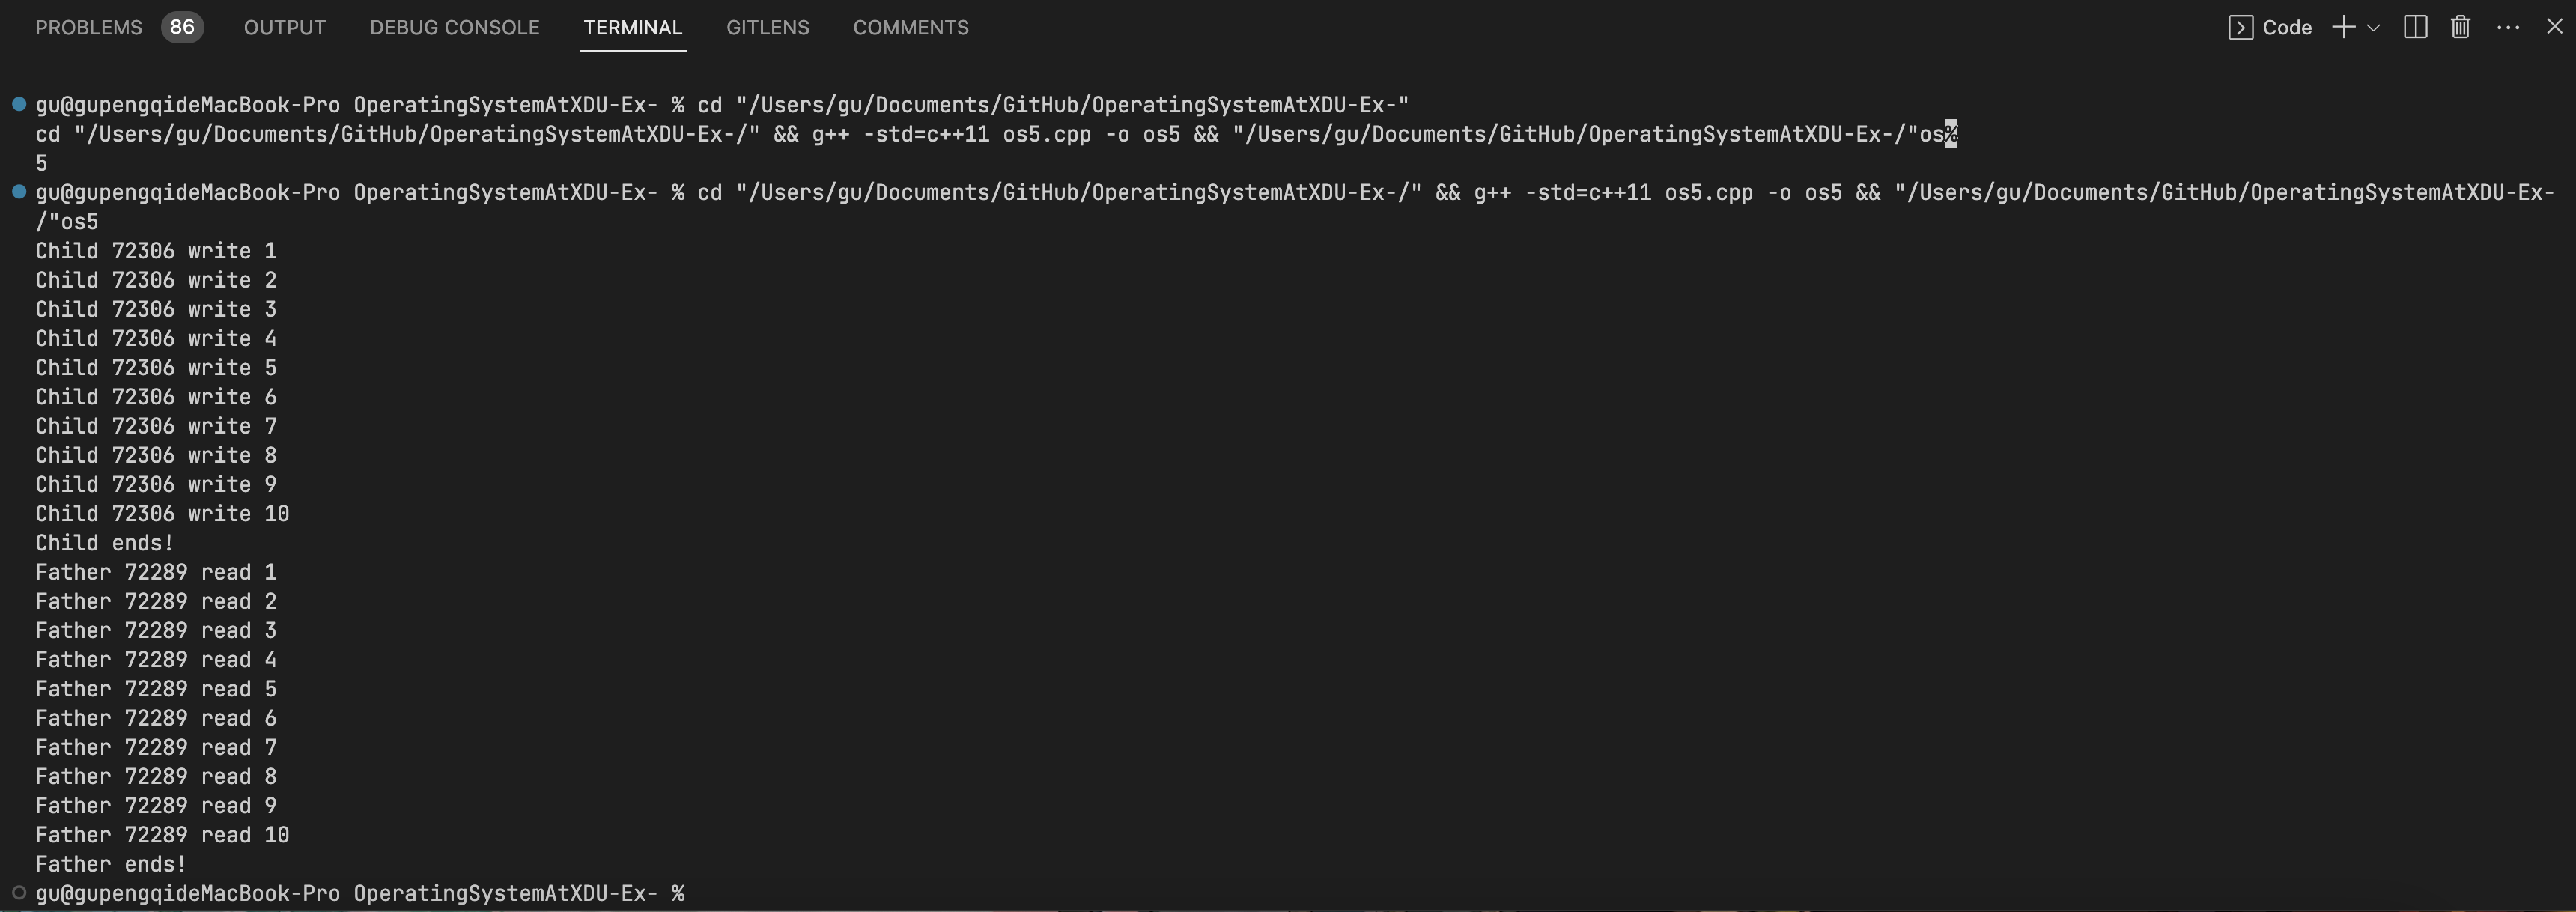
\includegraphics[width=0.8\pdfpagewidth]{os5.png}
	\end{center}
\end{figure}
\subsection{实验结果分析}
父进程率先创建了命名匿名管道\texttt{PATH}。子进程将测试数据1至10有序写入了该管道(因为\texttt{sleep}函数,连续两次写入完成s输出之间存在时间间隔),并在最终留下“\textit{Fin.}”作为数据结束暗示。父进程读取这些数据并输出出来,在读取到“\textit{Fin.}”后停止读取(输出“\textit{Father ends!}”),此次命名匿名管道通信完成。
\subsection{反思·心得}
文件的本质是流,因此理论上也可以利用文件系统来维护多个进程之间的通信管道。
\end{document}